\documentclass[8pt,letterpaper]{article}
\usepackage{graphicx}

\begin{document}
\title{A random walker world map generator}
\maketitle

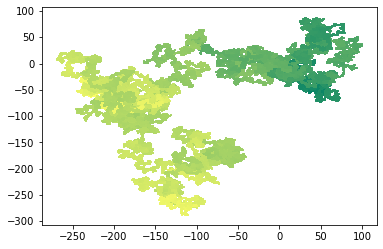
\includegraphics{Images/random_walker_world.png}
\newpage{}
\section{Introduction}
The random walker algorithm is created with the goal to create a random movement generator. by marking the spots where the walker has visited a world map can be generated in a simple way. The walker used in this test is a 3d walker. The first two dimensions(x and y axis) are used to create a 2d map. The 3rd dimension is used to create color in the map.
\section{The advantages}
The advantages of the random walker are:
\begin{itemize}
    \item A fast method to create worlds
        \begin{itemize}
        \item Fast loading times;
        \item Easy to create;
        \item Low processor power required.
        \end{itemize}
    \item simple but nice looking worlds
\end{itemize}
\section{The disadvantages}
The disadvantages of the random walker are
\begin{itemize}
    \item low adaptability
    \item no control over world generation
    \item Changing sprite work is near impossible
\end{itemize}

\section{conclusion}
The method is fun for simple world generation but is not usable for how advanced I want the world creator to be, therefore this method will not be used in the last version. Perlin noise might have similarities with this method that will be used in later versions of this generator.

\end{document}



